
\documentclass[border=10pt, 12pt]{standalone}
\usepackage[svgnames]{xcolor}
\usepackage{amsmath}
\usepackage{pgfplots}
\pgfplotsset{compat=newest}
\usepackage[sfdefault]{FiraSans}
\usepackage{FiraMono}
\renewcommand*\familydefault{\sfdefault}
\begin{document}
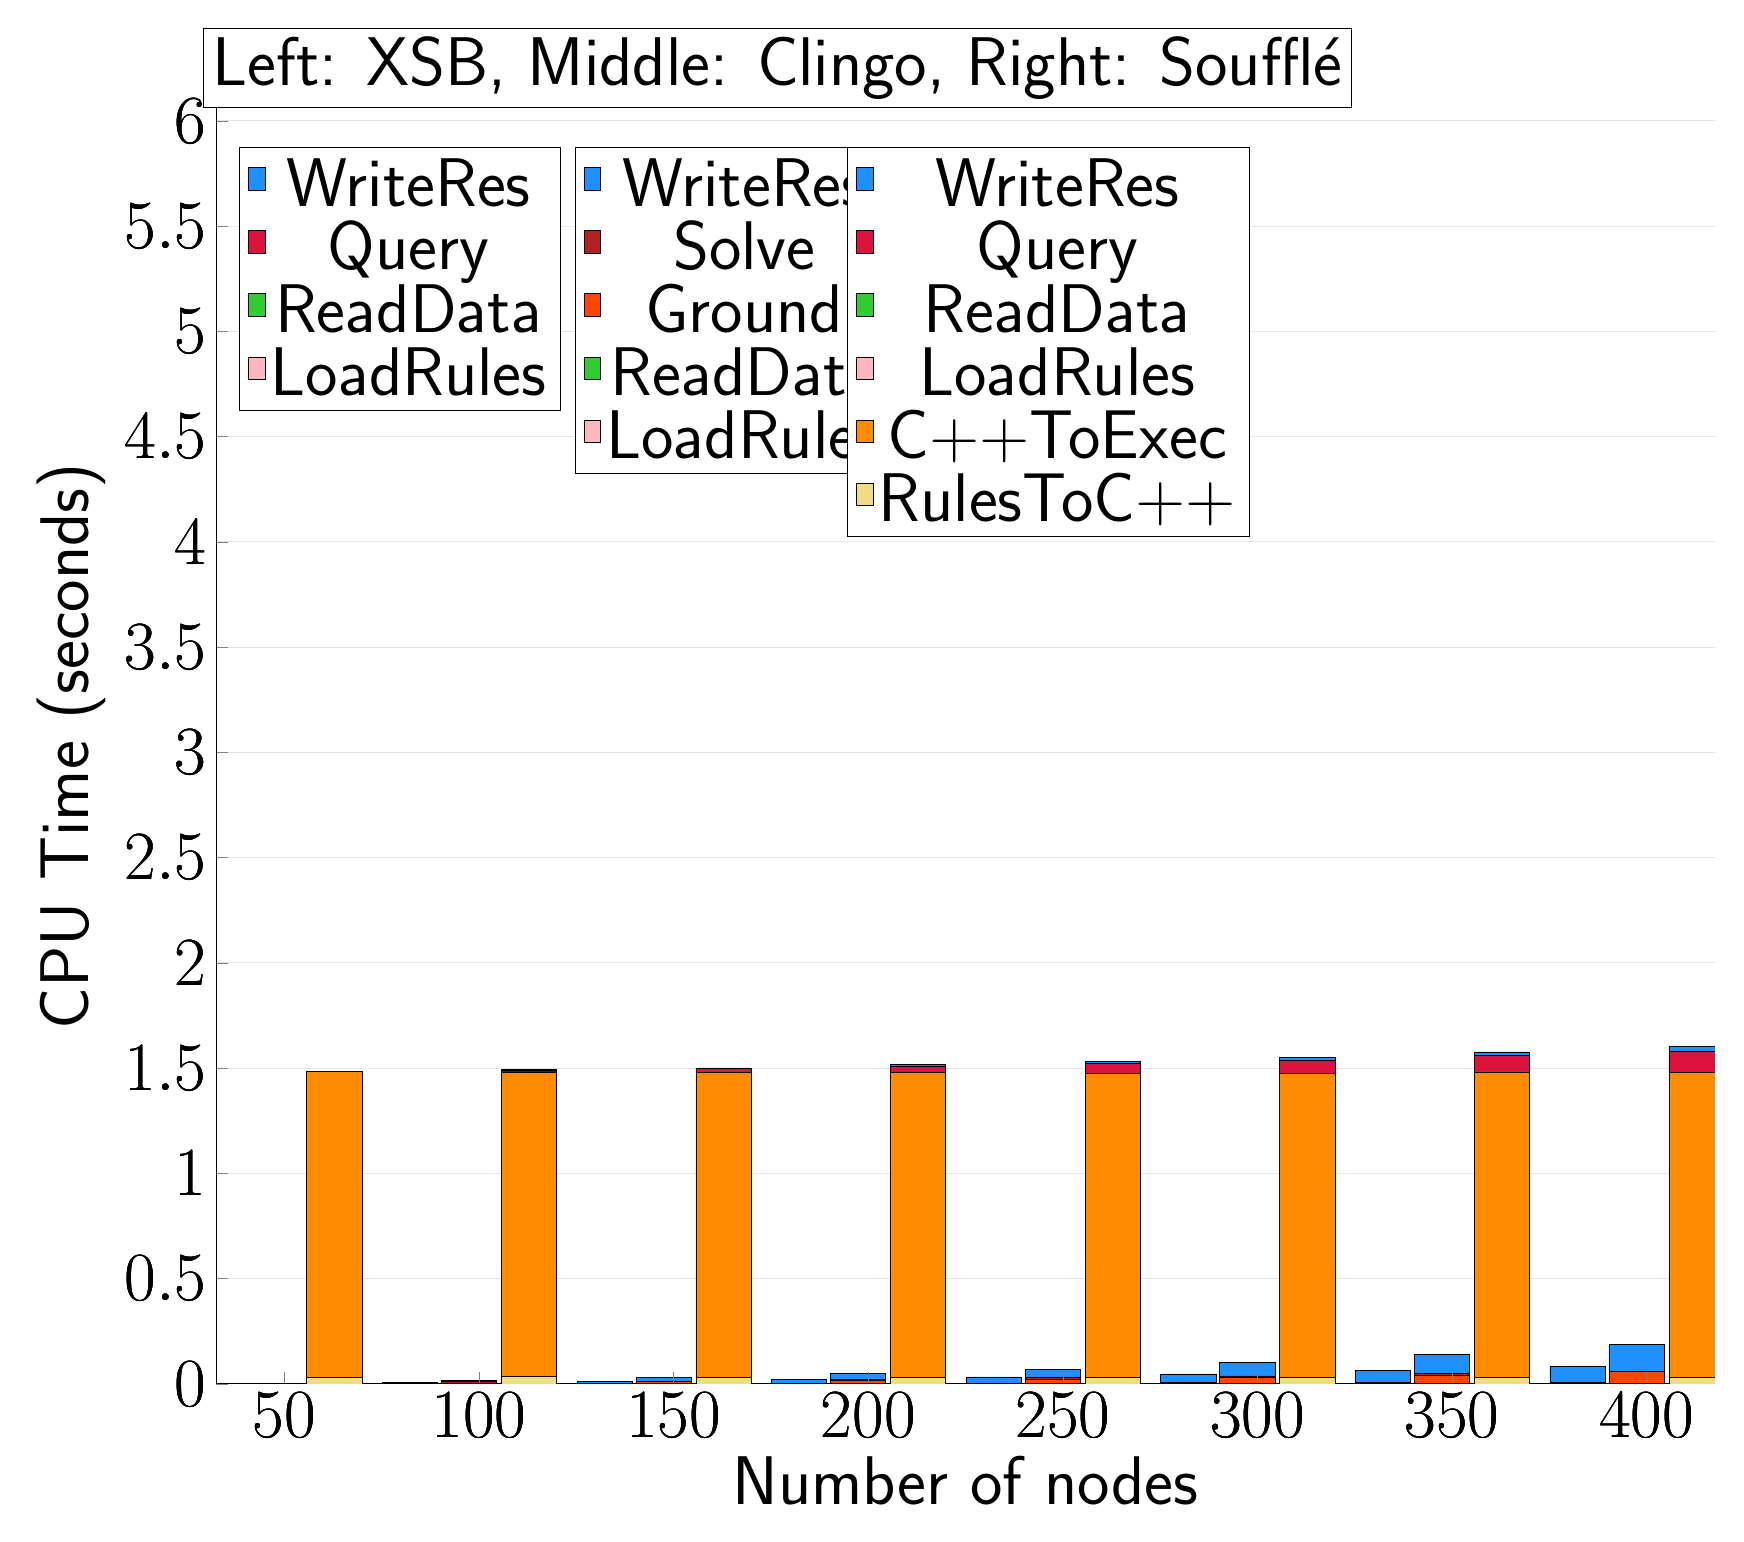
\begin{tikzpicture}
	\begin{axis}[bar shift=-25pt,
			ybar stacked,
			width=1.7\textwidth,
			bar width=0.7cm,
			ymajorgrids, tick align=inside,
			major grid style={draw=gray!20},
			xtick=data,
			ymin=0, ymax=6.059334,
			axis x line*=bottom,
			axis y line*=left,
			enlarge x limits=0.05,
			legend style={
					at={(0.23, 0.97)},
					anchor=north east,
					legend columns=1,
					font=\Huge,
				},
			ylabel={CPU Time (seconds)},
			xlabel={Number of nodes},
			label style={font=\Huge},
			tick label style={font=\Huge},
		]
		\addlegendimage{fill=DodgerBlue, draw=black, line width=0.2pt}
		\addlegendentry{WriteRes}
		\addlegendimage{fill=Crimson, draw=black, line width=0.2pt}
		\addlegendentry{Query}
		\addlegendimage{fill=LimeGreen, draw=black, line width=0.2pt}
		\addlegendentry{ReadData}
		\addlegendimage{fill=LightPink, draw=black, line width=0.2pt}
		\addlegendentry{LoadRules}
		\addplot +[fill=LightPink, draw=black, line width=0.2pt] coordinates {
				(50, 0.0006029999999999999)
				(100, 0.0006035000000000003)
				(150, 0.0006086000000000005)
				(200, 0.0006151000000000002)
				(250, 0.0005991000000000003)
				(300, 0.0006162999999999996)
				(350, 0.0006131999999999998)
				(400, 0.0006004000000000001)
			};
		\addplot +[fill=LimeGreen, draw=black, line width=0.2pt] coordinates {
				(50, 0.0001740999999999999)
				(100, 0.000215)
				(150, 0.0002636999999999997)
				(200, 0.0003121000000000001)
				(250, 0.0003459999999999999)
				(300, 0.00039950000000000066)
				(350, 0.0004341999999999993)
				(400, 0.0004806999999999998)
			};
		\addplot +[fill=Crimson, draw=black, line width=0.2pt] coordinates {
				(50, 0.00012520000000000022)
				(100, 0.0004805000000000008)
				(150, 0.0010642999999999998)
				(200, 0.0018938)
				(250, 0.0029652000000000003)
				(300, 0.0042975999999999995)
				(350, 0.006340799999999999)
				(400, 0.008348499999999998)
			};
		\addplot +[fill=DodgerBlue, draw=black, line width=0.2pt] coordinates {
				(50, 0.0011692999999999999)
				(100, 0.004517799999999999)
				(150, 0.0103823)
				(200, 0.0184286)
				(250, 0.0288118)
				(300, 0.0414263)
				(350, 0.056022300000000004)
				(400, 0.0739252)
			};
	\end{axis}

	\begin{axis}[bar shift=-3.7pt,
			ybar stacked,
			width=1.7\textwidth,
			bar width=0.7cm,
			ymajorgrids, tick align=inside,
			major grid style={draw=none},
			xtick=data,
			ymin=0, ymax=6.059334,
			axis x line*=none,
			axis y line*=none,
			enlarge x limits=0.05,
			legend style={
					at={(0.454, 0.97)},
					anchor=north east,
					legend columns=1,
					font=\Huge,
				},
			label style={font=\Huge},
			tick label style={font=\Huge},
		]
		\addlegendimage{fill=DodgerBlue, draw=black, line width=0.2pt}
		\addlegendentry{WriteRes}
		\addlegendimage{fill=FireBrick, draw=black, line width=0.2pt}
		\addlegendentry{Solve}
		\addlegendimage{fill=OrangeRed, draw=black, line width=0.2pt}
		\addlegendentry{Ground}
		\addlegendimage{fill=LimeGreen, draw=black, line width=0.2pt}
		\addlegendentry{ReadData}
		\addlegendimage{fill=LightPink, draw=black, line width=0.2pt}
		\addlegendentry{LoadRules}
		\addplot +[fill=LightPink, draw=black, line width=0.2pt] coordinates {
				(50, 0.0)
				(100, 0.0)
				(150, 0.0)
				(200, 0.0)
				(250, 0.0)
				(300, 0.0)
				(350, 0.0)
				(400, 0.0)
			};
		\addplot +[fill=LimeGreen, draw=black, line width=0.2pt] coordinates {
				(50, 0.0)
				(100, 0.0)
				(150, 0.0)
				(200, 0.0)
				(250, 0.0)
				(300, 0.0)
				(350, 0.0)
				(400, 0.0)
			};
		\addplot +[fill=OrangeRed, draw=black, line width=0.2pt] coordinates {
				(50, 0.0)
				(100, 0.0019999999999999996)
				(150, 0.009999999999999997)
				(200, 0.018)
				(250, 0.019999999999999997)
				(300, 0.030000000000000006)
				(350, 0.03999999999999999)
				(400, 0.05800000000000001)
			};
		\addplot +[fill=FireBrick, draw=black, line width=0.2pt] coordinates {
				(50, 0.0)
				(100, 0.007999999999999997)
				(150, 0.0)
				(200, 0.0020000000000000005)
				(250, 0.009000000000000003)
				(300, 0.007999999999999997)
				(350, 0.010000000000000009)
				(400, 0.001999999999999999)
			};
		\addplot +[fill=DodgerBlue, draw=black, line width=0.2pt] coordinates {
				(50, 0.0009999999999999998)
				(100, 0.007999999999999997)
				(150, 0.020000000000000007)
				(200, 0.028000000000000004)
				(250, 0.039999999999999994)
				(300, 0.06400000000000002)
				(350, 0.08799999999999998)
				(400, 0.12800000000000003)
			};
	\end{axis}

	\begin{axis}[bar shift=18pt,
			ybar stacked,
			width=1.7\textwidth,
			bar width=0.7cm,
			ymajorgrids, tick align=inside,
			major grid style={draw=none},
			xtick=data,
			ymin=0, ymax=6.059334,
			axis x line*=none,
			axis y line*=none,
			enlarge x limits=0.05,
			legend style={
					at={(0.69, 0.97)},
					anchor=north east,
					legend columns=1,
					font=\Huge,
				},
			label style={font=\Huge},
			tick label style={font=\Huge},
		]
		\addlegendimage{fill=DodgerBlue, draw=black, line width=0.2pt}
		\addlegendentry{WriteRes}
		\addlegendimage{fill=Crimson, draw=black, line width=0.2pt}
		\addlegendentry{Query}
		\addlegendimage{fill=LimeGreen, draw=black, line width=0.2pt}
		\addlegendentry{ReadData}
		\addlegendimage{fill=LightPink, draw=black, line width=0.2pt}
		\addlegendentry{LoadRules}
		\addlegendimage{fill=DarkOrange, draw=black, line width=0.2pt}
		\addlegendentry{C++ToExec}
		\addlegendimage{fill=LightGoldenrod, draw=black, line width=0.2pt}
		\addlegendentry{RulesToC++}
		\addplot +[fill=LightGoldenrod, draw=black, line width=0.2pt] coordinates {
				(50, 0.030000000000000006)
				(100, 0.034)
				(150, 0.030000000000000006)
				(200, 0.030000000000000006)
				(250, 0.030000000000000006)
				(300, 0.030000000000000006)
				(350, 0.030000000000000006)
				(400, 0.030000000000000006)
			};
		\addplot +[fill=DarkOrange, draw=black, line width=0.2pt] coordinates {
				(50, 1.453)
				(100, 1.4479999999999997)
				(150, 1.4499999999999997)
				(200, 1.45)
				(250, 1.4449999999999998)
				(300, 1.4449999999999998)
				(350, 1.4509999999999998)
				(400, 1.4479999999999997)
			};
		\addplot +[fill=LightPink, draw=black, line width=0.2pt] coordinates {
				(50, 9.35e-05)
				(100, 0.00010080000000000002)
				(150, 8.66e-05)
				(200, 0.00012230000000000002)
				(250, 0.00012340000000000002)
				(300, 0.00012200000000000001)
				(350, 7.48e-05)
				(400, 8.53e-05)
			};
		\addplot +[fill=LimeGreen, draw=black, line width=0.2pt] coordinates {
				(50, 0.0003187)
				(100, 0.000437)
				(150, 0.0005239)
				(200, 0.0006938999999999999)
				(250, 0.0007925999999999999)
				(300, 0.0008845000000000001)
				(350, 0.0009070999999999999)
				(400, 0.0010073)
			};
		\addplot +[fill=Crimson, draw=black, line width=0.2pt] coordinates {
				(50, 0.0016471000000000003)
				(100, 0.0079314)
				(150, 0.0163472)
				(200, 0.0300908)
				(250, 0.0450924)
				(300, 0.061938400000000005)
				(350, 0.07762260000000001)
				(400, 0.1010922)
			};
		\addplot +[fill=DodgerBlue, draw=black, line width=0.2pt] coordinates {
				(50, 0.0007196)
				(100, 0.0022819)
				(150, 0.0043135)
				(200, 0.006930400000000001)
				(250, 0.009600599999999999)
				(300, 0.012846100000000003)
				(350, 0.017316900000000003)
				(400, 0.0226209)
			};
	\end{axis}


	\node[anchor=south, draw, fill=white] at (rel axis cs:0.42,1) {\Huge Left: XSB, Middle: Clingo, Right: Soufflé};
\end{tikzpicture}
\end{document}
